% THIS IS AN EXAMPLE DOCUMENT FOR VLDB 2012
% based on ACM SIGPROC-SP.TEX VERSION 2.7
% Modified by  Gerald Weber <gerald@cs.auckland.ac.nz>
% Removed the requirement to include *bbl file in here. (AhmetSacan, Sep2012)
% Fixed the equation on page 3 to prevent line overflow. (AhmetSacan, Sep2012)

\documentclass[sigconf, nonacm]{acmart}
\usepackage{graphicx}
\usepackage{balance}  % for  \balance 
\usepackage{graphics}
\usepackage{mdwlist}


% Include information below and uncomment for camera ready
%\vldbTitle{}
%\vldbAuthors{}
%\vldbDOI{}
%\vldbVolume{}
%\vldbNumber{}
%\vldbYear{}

\begin{document}

\newcommand{\beq}{\begin{equation}}
	\newcommand{\eeq}{\end{equation}}
\newcommand{\bit}{\begin{itemize*}}
	\newcommand{\eit}{\end{itemize*}}
\newcommand{\goal}[1]{ {\noindent {$\Rightarrow$} \em {#1} } }
\newcommand{\hide}[1]{}
%\newcommand{\comment}[1]{ {\footnotesize {#1} } }
%\newtheorem{lemma}{Lemma}
%\newtheorem{theorem}{Theorem}
%\newtheorem{proof}{Proof}
%\newtheorem{defn}{Definition}
%\newtheorem{algo}{Algorithm}
%\newtheorem{observation}{Observation}

% ****************** TITLE ****************************************

\title{Recipe Prediction and Completion with Attentioned Multipartite Network}

%\numberofauthors{3} 

\author{Daeho Lee}
\affiliation{
  \institution{Graduate School of BBE, KAIST}
  \city{Daejeon}
  \state{South Korea}
}
\email{daeho715@kaist.ac.kr}

\author{Sang Un Gu}
\affiliation{
    \institution{Kim Jaechul Graduate School of AI, KAIST}
    \city{Daejeon}
    \state{South Korea}
}
\email{ayslaon311@kaist.ac.kr}

\author{Youngjun Im}
\affiliation{
    \institution{School of Computing, KAIST}
    \city{Daejeon}
    \state{South Korea}
}
\email{carol@kaist.ac.kr}
    
\begin{abstract}
	This project is about prediction and completion task of given 35317 recipes, 6714 ingredients and 20 cuisines. To handle these tasks, we decided to use recommendation system. Recently, with applying neural network methods into graph structures, especially graph convolutional networks(GCN) give the best performance in the recommendation tasks. However, many graph neural networks were lack of scalability due to the ineffectiveness of Laplacian matrix. To handle this issue, works such as PinSAGE and MultiSAGE based on random-walk have been done. 

In our task, there is need to consider connectivity of ingredients and cuisines represented as recipes. Therefore, we need to consider the graph which can understand the contexts; recipes. So we decided to construct heterogeneous graph consisting of three types of nodes of ingredients, recipes and cuisines rather than bi-partite graph in PinSAGE. We'll follow the contextualized multi embeddings in MultiSAGE expected to be able to consider importance of the weights in connected nodes.
\end{abstract}
\maketitle

\section{Introduction}
\label{sec:intro}
Predicting cuisine from ingredients is to solve the completion task and classification task by using 6714 ingredients, 35317 recipes, and 20 cuisines.
The completion task is to find a missing ingredient in a given recipe.
The classification task is to find cuisine using a perfect recipe.
The completion task predicts missing ingredients, so it can be helpful for grocery shopping or cooking at home.
The classification task predicts the cuisine for each recipe, so it can know ingredients that are frequently used in a particular cuisine.
Therefore, it can be helpful in trade or exchange by each country.

We decided to use a recommendation system to solve these problems.
A \emph{recommendation system} is a tool that assists users by presenting services or products that are most likely of their interest.
In general, recommendations can be generated based on user preferences, item features, user-item transactions, and environmental factors such as time, season, and location.[1]

Recently, the best performance of the recommendation system is the graph neural network, one of the deep learning architectures.
Among graph neural networks, convolutional neural networks (GCNS) have received significant attention for the task of extracting information from large graphs.[2] 

GraphSAGE (SAmple and agreGate)[3] was created for inductive learning of GCNS.
GraphSAGE trains a set of aggregator functions that learn to aggregate feature information from a node's local neighborhood.
Among the recommendation system based on GraphSAGE are PinSAGE and  MultiSAGE.

PinSAGE[4] is a random-work-based GCN. In PinSAGE, Pin and Board are expressed in a bipartite graph.
The Pin is a general item, and the board represents multiple pins.
Personalized Pagerank algorithm(PPR)[5] can be utilized as high-order heuristics that consider neighbors of the target node in the whole network for calculating the similarity score.
The aggregate in PinSAGE used a PPR.
PinSAGE captures connection information between pins through Metapath(Pin-Board-Pin) and embedding only for pins.
Thus, PinSAGE considers the graph to be a homogeneous network of the Pin.
Since the information on the board is used only as a metapath, there is a disadvantage in embedding information of node types other than the Pin cannot be generated.

PPR is a pooling score that does not reflect the feature information of nodes.
Thus, MultiSAGE[6] introduces the concept of graph attention network(GAT)[7].
Also, unlike PinSAGE, which created and learned graphs in the form of bi-partite, MultiSAGE enables contextualized multi embeddings.
That is, The embedding type can be different according to the situation.

If a graph is made using the connectivity of ingredients, recipes, and cuisines in the predicting cuisine problem, it becomes a heterogeneous network with three types of nodes.
Therefore, if each node is practiced as an essential weight of a connected node through node embedding of MultiSAGE, it will perform well in the completion task and classification task.


%\section{Survey}
%\label{sec:survey}
%Next we list the papers that each member read,
along with their summary and critique.
Table \ref{tab:symbols} gives a list of common symbols we used.

\begin{table}[htb]
\begin{center} 
\begin{tabular}{|l | c | } \hline \hline 
Symbol & Definition \\ \hline
$N$ & number of sound-clips \\
$D$ & average duration of a sound-clip \\
$k$  & number of classes \\ \hline
\end{tabular} 
\end{center} 
\caption{Symbols and definitions}
\label{tab:symbols} 
 \end{table} 


\subsection{Papers read by John Smith}
The first paper was the wavelet paper by Daubechies
\cite{Daubechies92Ten}
\begin{itemize*}
\item {\em Main idea}: instead of using Fourier transform,
      wavelet basis functions are localized in frequency {\em and} time.
      It turns out that they fit real signals better,
      in the sense they need fewer non-zero coefficients to reconstruct
      them. Thus they achieve better compression.
\item {\em Use for our project}:
      it is extremely related to our sound-clip similarity
      project, because we can use the top few wavelet coefficients
      to compare two sound clips.
\item {\em Shortcomings}:
      The Daubechies wavelets require a wrap-around setting,
      which may lead to non-intuitive results.
\end{itemize*}

The second paper was by $\ldots$

The third paper was by $\ldots$

\subsection{Papers read by Mary Thompson }

$\ldots$

\subsection{Papers read by  Michael Miller }

$\ldots$


\section{Proposed Method}
\label{sec:proposed}
\subsection{Preliminaries}

The three types of attributes exist in the graph.
\bit
    \item Node attributes (e.g., node identity, number of neighbors)
    \item Edge attributes (e.g., edge identity, edge weights)
    \item Global attributes (e.g., number of nodes, longest path)
\eit
The objective of the project is to complete recipes and classify cuisine aligns with learning attributes of nodes, especially those of ingredients.
The provided dataset possesses an apparent heterogeneity as visualized in Figure \ref{fig:tripartite}.
In the graph's global scope, ingredient nodes can be considered target nodes, while recipe nodes and cuisine nodes can be considered context nodes.

\begin{figure}[btp!]
    \centering
    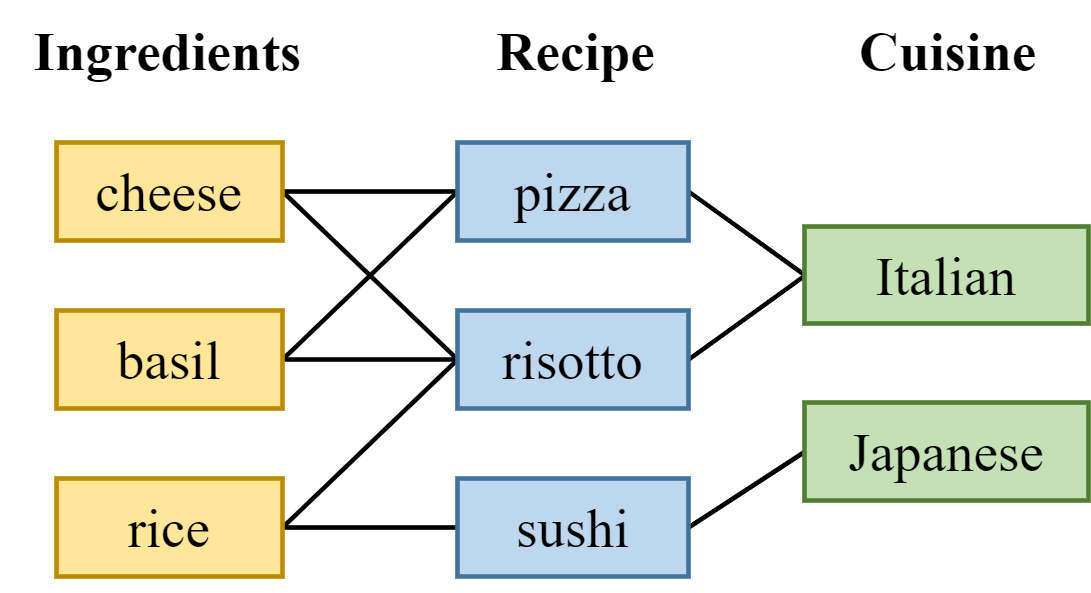
\includegraphics[width=0.6\linewidth]{FIG/tripartite.png}
    \caption{\label{fig:tripartite}Simplified example of constructed graph.}
\end{figure}

\subsection{MultiSAGE}

Our method includes the idea from MultiSage, a graph convolutional network for a recommender system.
The MultiSAGE\cite{10.1145/3394486.3403293} is a GCN engine with contextual information, modeling interactions between target nodes and context nodes in the multipartite network.
The key improvements of MultiSAGE from PinSAGE are \emph{contextual masking} and \emph{contextual attention}.

Contextual masking aggregates the target embeddings $\mathbf{z}_t$ based on context embeddings $\mathbf{z}_c$ as following equation.
\begin{equation}
    \mathbf{z}_{t|c} = \mathbf{z}_t \otimes \mathbf{z}_c
\end{equation}
Since the last embedding layer of $\mathbf{z}_c$ is the ReLU activation function, which sets dimensions with negative values as zeros, the target embeddings' irrelevant dimension is masked out by the corresponding context. This relational operation has intuitive geometrical meanings, and has shown empirical predominancy over popular operations such as summation $\mathbf{z}_t \oplus \mathbf{z}_c$ and dense neural network $\text{RELU}(\mathbf{W}_p(\mathbf{z}_t \otimes \mathbf{z}_c) + \mathbf{b}_p)$.

Contextual attention accounts for the context-wise dynamic impact of neighbor nodes with regard to the ego node. The attention of edge is jointly computed by the ego-context-neighbor relationship as follows.
\begin{equation}
\begin{split}
    & \alpha(v, o, u) = \\
    & \frac{\exp\left(\tau(\mathbf{a}^T[\mathbf{W}_{at}\mathbf{z}_t(v) \odot \mathbf{W}_{ac}\mathbf{z}_c(o) \odot \mathbf{W}_{at}\mathbf{z}_t(u)])\right)}{\sum\limits_{\substack{u' \in \mathcal{N}_v,\\o' \sim (v, u')}}\exp\left(\tau(\mathbf{a}^T[\mathbf{W}_{at}\mathbf{z}_t(v) \odot \mathbf{W}_{ac}\mathbf{z}_c(o') \odot \mathbf{W}_{at}\mathbf{z}_t(u')])\right)}
\end{split}
\end{equation}
Here, $\mathbf{W}_{at}$ and $\mathbf{W}_{ac}$ are the learnable parameters for target embedding and context embedding, respectively. The multi-head attention mechanism is used to aggregate contextualized embedding as follows:
\begin{equation}
    \mathbf{z}_{\mathcal{N}_v}(x) = \sigma \left( \frac{1}{D} \sum_{d=1}^{D} \sum_{u \in \mathcal{N}_v, o \sim (v, u)} \alpha^{(d)}(v, o, u) \mathbf{z}_{t|c}(x, o) \right),
\end{equation}
where $\sigma$ is a sigmoid function.

The training objective is a max-margin ranking described as follows,
\begin{equation}
    \mathcal{J}(v_q, v_p, v_n) = \max\{ 0, \mathbf{h}_{v_q}^T \mathbf{h}_{v_n} - \mathbf{h}_{v_q}^T \mathbf{h}_{v_p} + \delta \},
\end{equation}
where $\delta$ is a margin hyper-parameter. The $v_q, v_p, v_n$ corresponds to the query node, positive node and negative node, respectively, sampled from the training data.

The advances of this project from the original MultiSAGE algorithm are three-fold.
\bit
    \item We empirically demonstrate the claim in \cite{10.1145/3394486.3403293} that MultiSAGE can incorporate multiple context types simultaneously during the training and testing phase.
    \item Furthermore, we extend the \emph{level} of context nodes and show that indirect contexts are also effective for learning target features. For example, as depicted in Figure \ref{fig:tripartite}, we utilize indirect context \textit{cuisine} that are not directly connected to target node \textit{ingredients}.
    \item We extend the architecture to perform collaborative filtering and classification over the learned node embeddings.
\eit

\subsection{Graph construction}

\begin{table}[btp!]
    \centering
    \begin{tabular}{ l r l r }
        \toprule
        \multirow{3}{*}{$|V|$} & \multirow{3}{*}{30281}  & $|V_{I}|$  & 6714   \\
                               &                         & $|V_{R}|$  & 23547  \\
                               &                         & $|V_{C}|$  & 20     \\
        \midrule
        \multirow{2}{*}{$|E|$} & \multirow{2}{*}{277006} & $|E_{IR}|$ & 253459 \\
                               &                         & $|E_{RC}|$ & 23547  \\
        \bottomrule
    \end{tabular}
    \caption{\label{tab:graph_size}Some statistics of graph. $|V|$ and $|E|$ are number of nodes and edges in the graph, respectively. $|V_{I}|, |V_{R}|, |V_{C}|$ are number of nodes with type \textit{ingredient}, \textit{recipe}, \textit{cuisine}, respectively. $|E_{IR}|, |E_{RC}|$ are edges between ingredient and recipe, recipe and cuisine, respectively.}
\end{table}

Alongside the structure of the graph, the method for the generation of initial node features is an interesting topic.
Since the name of every ingredient is given, one might use the NLP-based algorithms to extract feature-based embeddings.
However, because given names are relatively short and the graph consists of a relatively small number of nodes, using identity-based embedding is practical and simplifies the network.

% To discuss:
% \subsection{Recipe completion task}
% \subsection{Cuisine classification task}



\section{Experiments}
\label{sec:experiments}


 We conduct experiments on given dataset which consists of 35317 recipes, 6714 ingredients and 20 cuisines. In following sections, we would compare our results and some results from basic models such as Random Forest, Linear Regression, and Linear SVC.
 
 \subsection{Dataset}
 Dataset consists of 7 files. \texttt{train.csv} has 35317 rows where each row represents the recipe. \texttt{validation\_\texttt{\{classification/completion\}}\_\texttt{\{answer/question\}}.csv} has 7847 rows for each tasks. \texttt{test\_\texttt{\{classification/completion\}}\_question.csv} has 3923 rows for each tasks and the test set has no answers.  
 
  We're aiming to train the MultiSAGE model suggested to solve the given tasks with \texttt{train.csv} and validate the performance of model with \texttt{validation*.csv} files and submit the answers of the test set.

  The class distributions of the train and validation set are shown in figure \autoref{fig:class_dist}, respectively.

  \begin{figure}
      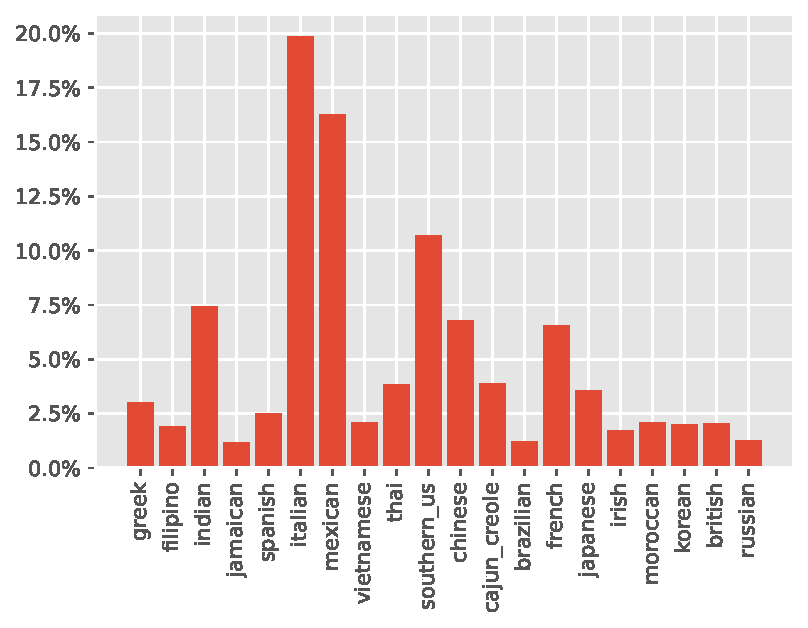
\includegraphics[width=0.49\linewidth]{FIG/train_class_dist.pdf}
      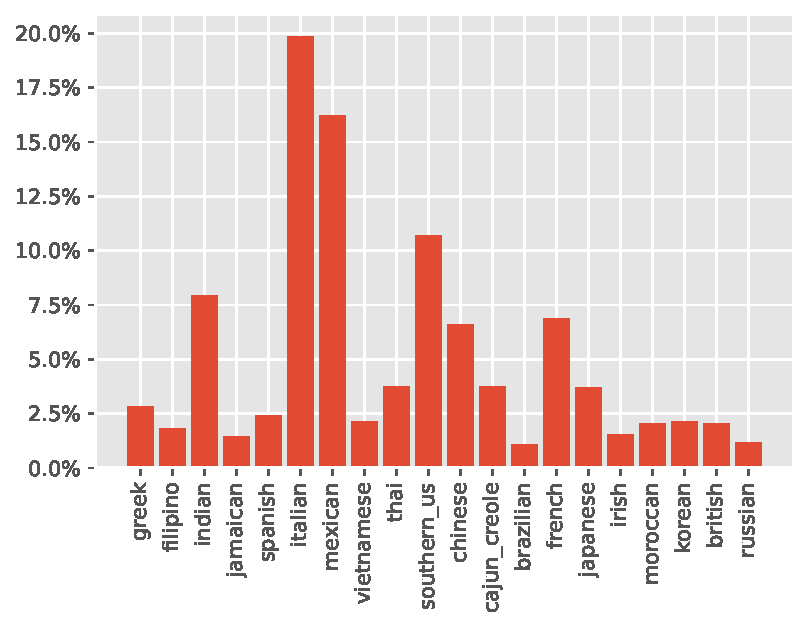
\includegraphics[width=0.49\linewidth]{FIG/val_class_dist.pdf}
      \caption{\label{fig:class_dist} Class distribution of the training set (left) and validation set (right).}
  \end{figure}

 \subsection{Recipe Classification Task Into Cuisine}

 \begin{table}[btp!]
    \centering
    \resizebox{\linewidth}{!}{%
    \begin{tabular}{ c c c c }
        \toprule
        \textbf{Methods} & \textbf{Micro F1-score} & \textbf{Macro F1-score} & \textbf{Accuracy} \\
        \midrule
        LinearSVC & 0.635 & 0.510 & 0.635 \\
        RandomForest & 0.471 & 0.210 & 0.472 \\
        Linear Regression & 0.638 & 0.531 & 0.638 \\
        \textbf{MultiSAGE} & 0.615 & 0.455 & 0.616 \\
        \bottomrule
        
    \end{tabular}
    }
    \caption{\label{tab:classification_task_result} Performance measured by \{Micro/Macro\} F1-score and accuracy of each model in validation classification set.}

 \end{table}
 
  The results of classification on validation set using our model and other baseline models are shown in \autoref{tab:classification_task_result}.  
  We used the classification method using 6714 ingredient node vectors learned through MultiSAGE. Through MultiSAGE, the ingredient node learned recipe information through context vector. Each ingredient node was trained as a 256-dimensional vector. A single representative node was created through the mean method of aggregation by selecting a vector for the ingredients of the recipe. 20 cuisines were predicted using this 256-dimensional vector. As a result, multiSAGE performed better than other models.
  
 \subsection{Ingredient Completion Task}
 For the completion task, we computed the sum of pairwise score between the ingredients already in the recipe $R$ and the new ingredient $i$. The missing ingredient can be found by choosing the ingredient that maximizes the pairwise score.
 \begin{equation}
     Score(R, i) = \sum_{j \in R} \langle h_i, h_j \rangle + b_i + b_j.
 \end{equation}
 Here, $h$ is a node embedding and $b$ is a bias term learned by model's scoring function. See \texttt{completion.ipynb} for implementation details. The performance of the model for ingredient completion task is shown in Figure \autoref{fig:completion_val_ranks}.

 \begin{figure}[btp!]
     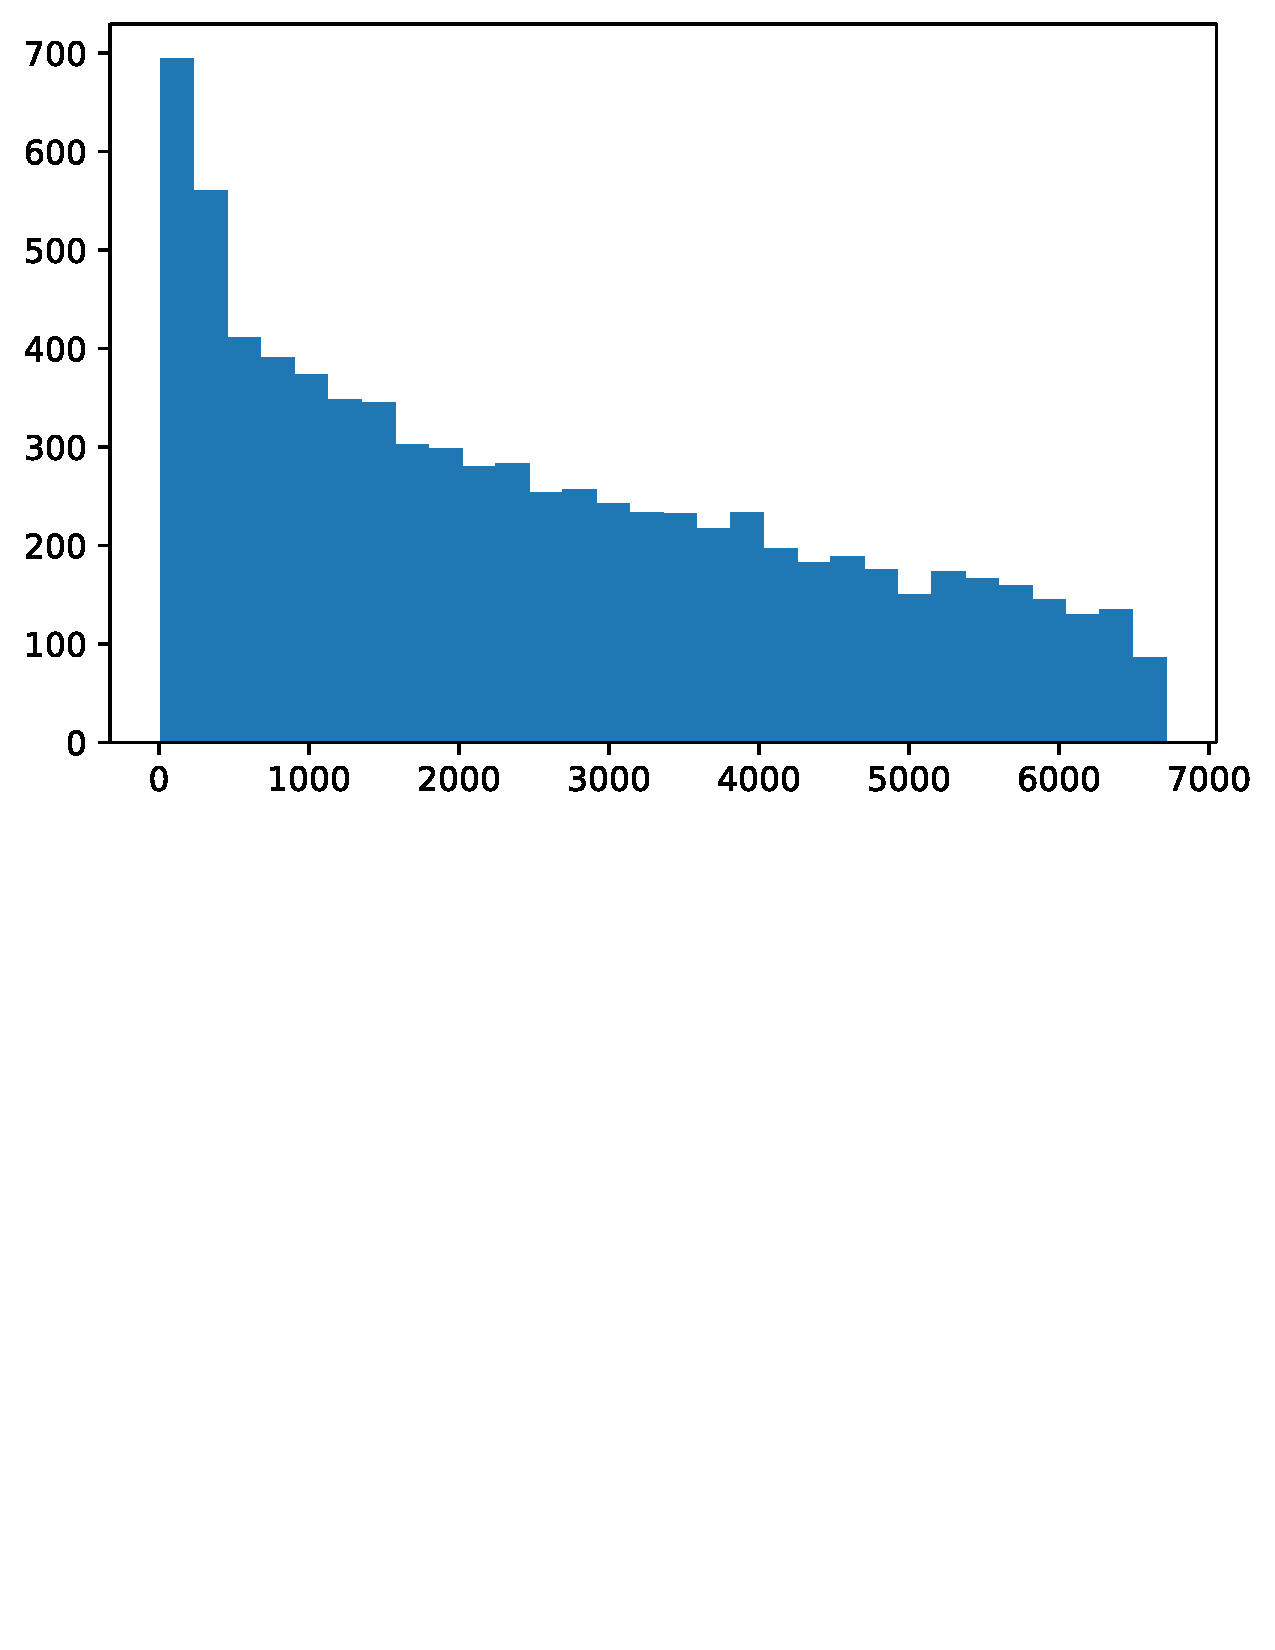
\includegraphics[width=\linewidth,trim={0 14cm 0 0},clip]{FIG/completion_val_ranks.pdf}
     \caption{\label{fig:completion_val_ranks} The rank distribution of the correct ingredient in the model's prediction.}
 \end{figure}

\begin{comment}
\begin{enumerate}
    \item MultiSAGE
    \begin{enumerate}
        \item Node Embedding
        \newline fig1 : heteogeneous node enbedding
        \item evaluate node Embedding
    \end{enumerate}
    \item Classification task
    \begin{enumerate}
        \item Evaluate models
        \newline fig2 models performance
    \end{enumerate}
    \item Completion task
    \begin{enumerate}
        \item Evaluate models
        \newline fig3 model performance
    \end{enumerate}
\end{enumerate}
\end{comment}



\section{Conclusions}
\label{sec:conclusions}
The proposed method {\em someMETHOD}
has the following advantages:
\bit
\item it gives better classification accuracy than all 10 competitors we tried
\item its accuracy is very close to the very best competitor
      in the {\em UCR Insect Classification Contest}.
\item it is scalable
\eit


\section{REFERENCES}
\label{sec:references}
[1]Da’u, Aminu, and Naomie Salim. "Recommendation system based on deep learning methods: a systematic review and new directions." Artificial Intelligence Review 53.4 (2020): 2709-2748.
\newline[2]Jie Chen, Tengfei Ma, and Cao Xiao. 2018. Fastgcn: fast learning with graph convolutional networks via importance sampling. In ICLR.
\newline[3] Hamilton, Will, Zhitao Ying, and Jure Leskovec. "Inductive representation learning on large graphs." Advances in neural information processing systems 30 (2017).
\newline[4] Ying, Rex, et al. "Graph convolutional neural networks for web-scale recommender systems." Proceedings of the 24th ACM SIGKDD international conference on knowledge discovery \& data mining. 2018.
\newline[5] Chowdhury A. Goel A. Bahmani, B. Fast incremental and personalized pagerank. Proceedings of the VLDB Endowment, 3(4):173–184, June 2010. 
\newline[6]Yang, Carl, et al. "Multisage: Empowering gcn with contextualized multi-embeddings on web-scale multipartite networks." Proceedings of the 26th ACM SIGKDD International Conference on Knowledge Discovery \& Data Mining. 2020.
\newline[7] Veličković, Petar, et al. "Graph attention networks." arXiv preprint arXiv:1710.10903 (2017).

\bibliographystyle{plain}

\newpage
\appendix
\section{Appendix}
\subsection{Labor Division}

The team will perform following tasks. The division of the labor and the tasks is subject to change.
\bit
\item Implementation of the multipartite graph [all]
\item Implementation of inference and training algorithm [all]
\item Experiments on the validation data [all]
\eit

\subsection{Full disclosure wrt dissertations/projects}

\paragraph{Daeho Lee:}
He is not doing any dissertation or project related to this project: he is in area of Bioinfomatics (drug discovery using AI).

\paragraph{Youngjun Im:}
He is not doing any dissertation or project related to this project: his research is on modeling point process using graph recurrent neural network.

\paragraph{Sang Un Gu:}
He is not doing any dissertation or project related to this project: he is in the area of explainable AI.




\end{document}
